% !TEX root = ../ac_paper.tex

\section{A Greedy Search Algorithm}

% Sketch of the section: We use search algorithm to get a baseline on results. We call it breadth-first search. It is able to solve less than half of the presentations we considered. We will use these presentations to generate dataset for each of the techniques used in the next two sections: for embeddings, we generate text dataset, for reinforcement learning, these states are the initial states of a Markov Decision Process. 

%\fixme{Made search space finite. Perhaps this could be discussed in the previous section. Justify the BFS name.}

In this section, we introduce a greedy search algorithm, referenced as \autoref{alg:bfs}, which bears resemblance to the A* search algorithm within the context of graph theory. The algorithm searches through the space of all balanced presentations, a path that connects an initial presentation $P_0$ to a trivial presentation. 
\newline 

$P_0$ is initially placed into a priority queue $Q$ and a set $S$. The priority queue is ordered by a tuple $(k, l)$ where $k$ is the total length of a presentation and $l$ is the path length between a state and $P_0$. The algorithm iteratively selects the top element from the priority queue and applies all possible AC moves to it to generate new states. If a state has not been seen before, the algorithm adds it to both $Q$ and $S$. This process is continued until the algorithm finds a trivial presentation, deeming the search process successful, or if it has seen a million distinct states. 
\newline

We put a cutoff of a million states to make the search process feasible within a practical timeframe. For 1190 presentations of the Miller-Schupp series, exploring a million states takes about 20 hours of CPU time. 
\footnote{Make sure this is correct.} We will call a presentation ``GS-easy" if the greedy search algorithm successfully finds a path that trivializes the presentation; otherwise, we will call it ``GS-hard". The distributions of ``GS-easy" and ``GS-hard" presentations as functions of $n$ and lengths of the presentations of the Miller-Schupp series is given in \fixme{Include reference.}

\begin{algorithm}
	\caption{Greedy Search Algorithm}\label{alg:bfs}
	\begin{algorithmic}
		\State $Q \gets P_0$ \Comment{Initialize the prioriy queue of presentations with $P_0$.}
		\State $S \gets P_0$ \Comment{Initialize the set of seen presentations with $P_0$.}

		\While{$\text{len}(S) < 10^6$} \Comment{While the number of distinct states is less than $10^6$.}
		\State $P \gets Q[0]$ \Comment{Pop the top element of the heap.}
		\For{$A \in \text{AC Moves}$}
		\State $PA \gets A \cdot P$ \Comment{Act on $P$ by $A$.}
		\If{PA is trivial}
		\Return{True}
		\Else{ $PA \notin S$}
		\State $S \gets PA$
		\State $Q \gets PA$ \Comment{Insert $PA$ to $Q$ with priority.}

		\EndIf
		\EndFor
		\EndWhile
	\end{algorithmic}
\end{algorithm}


\fixme{Start from here by plotting and including heatmaps.}

The number of BFS-hard examples increases as a function of $n$.
(See \autoref{fig:hist_vs_n}.)
The distributions of BFS-easy and BFS-hard as a function of the total length of a presentation are also given in \autoref{fig:hist_vs_length}.

%\begin{figure}
%	\centering
%	\begin{subfigure}[b]{0.5\textwidth}
%		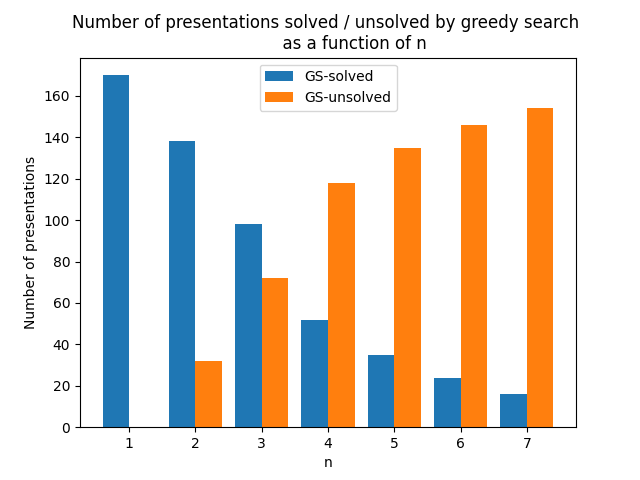
\includegraphics[width=\textwidth]{fig/hist_vs_n.png}
%		\caption{Distribution versus $n$}
%		\label{fig:hist_vs_n}
%	\end{subfigure}%
	%add desired spacing between images, e. g. ~, \quad, \qquad etc.
	%(or a blank line to force the subfigure onto a new line)
%	\begin{subfigure}[b]{0.5\textwidth}
%		\centering
%		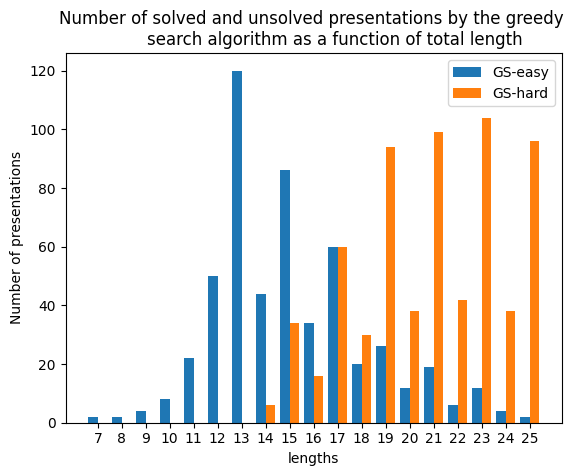
\includegraphics[width=\textwidth]{fig/hist_vs_lengths.png}
%		\caption{Distribution versus total length}
%		\label{fig:hist_vs_length}
%	\end{subfigure}
%	\caption{Number of presentations}\label{fig:miller_schupp_statistics}
%\end{figure}